% Naman's sections of the final report: E4, E5 and the discussion.
% Structure only. Every paragraph below is for Naman to write (the course
% requires the report text to be written by the team). Each TODO names the
% result file holding its facts; every number must match that file.
% Tables and figure: regenerate with `python scripts/final_assets.py`.

\section{Does the failure type decide the repair? (E4)}
\label{sec:e4}

% TODO (Naman): setup. What was re-asked (every value-question error of
% synthetic pilots 1 and 2: Qwen 631, LLaVA 1,015), the four repairs, how a
% repair counts as a recovery, and the pre-registered test.
% Facts: results/e4.md (Provenance), results/e4-preregistration.md.

% Generated by scripts/final_assets.py from results/e4/*.outcomes.jsonl
% Pilots 1 and 2 pooled; see results/e4.md. Caption: E4_CAPTION in the script.
\begin{table}[t]
\centering\small
\setlength{\tabcolsep}{3pt}
\begin{tabular}{lrcccc}
\toprule
Original answer & $n$ & Re-ask & Upsample & Crop & Verify \\
\midrule
\multicolumn{6}{l}{\textit{Qwen2.5-VL-7B}} \\
Misread & 46 & 0.11 & 0.13 & \textbf{0.26} & 0.09 \\
Made-up number & 91 & 0.00 & 0.00 & 0.00 & \textbf{0.14} \\
``0'' & 494 & 0.02 & 0.02 & 0.02 & \textbf{0.69} \\
\quad crop DiD & & \multicolumn{4}{c}{+0.261 [+0.140, +0.389]} \\
\midrule
\multicolumn{6}{l}{\textit{LLaVA-NeXT-7B}} \\
Misread & 415 & 0.03 & 0.01 & \textbf{0.15} & 0.03 \\
Made-up number & 368 & 0.00 & 0.00 & 0.00 & 0.00 \\
``0'' & 232 & 0.00 & 0.00 & 0.00 & 0.00 \\
\quad crop DiD & & \multicolumn{4}{c}{+0.152 [+0.119, +0.189]} \\
\bottomrule
\end{tabular}
\caption{E4 recovery rates on initially wrong value answers. Bold marks each
row's best repair, excluding zero ties. DiD compares crop's recovery gain on
misreads with its gain on made-up numbers. Brackets give 95\% CIs from figure
bootstraps; missing-bar ``0'' answers form a separate row.}
\label{tab:e4}
\end{table}


% TODO (Naman): result of the pre-registered test, both models (Table~\ref{tab:e4}).
% Facts: results/e4.md, Qwen and LLaVA sections.

% TODO (Naman): what limits the reading. Facts: results/e4.md,
% "Read these before writing them up", points 1 to 5.

\section{A type-aware controller (E5)}
\label{sec:e5}

% TODO (Naman): setup. The policies compared, how a re-look is priced on right
% answers (the re-ask of correct answers), cross-fitting by figure fold, AURC.
% Facts: results/e5.md, and src/controller/e5.py docstring for the method.

% Generated by scripts/final_assets.py from results/e5/*_e5.json
% (see results/e5.md). AURC: mean risk over the risk-coverage curve, lower
% is better; brackets are 95% cluster-bootstrap intervals.
% Caption: E5_CAPTION in the script.
\begin{table}[t]
\centering\small
\setlength{\tabcolsep}{3pt}
\begin{tabular}{lcc}
\toprule
Policy & AURC & 95\% CI \\
\midrule
\multicolumn{3}{l}{\textit{Qwen2.5-VL-7B}} \\
Plain model & 0.526 & [0.513, 0.538] \\
Binary abstention & 0.179 & [0.169, 0.190] \\
Missing-bar abstention & 0.208 & [0.191, 0.226] \\
Controller & 0.162 & [0.145, 0.180] \\
Re-look + binary & 0.114 & [0.103, 0.126] \\
Oracle & 0.056 & [0.049, 0.064] \\
\quad re-look gain (binary) & $-$0.065 & [$-$0.073, $-$0.056] \\
\quad re-look gain (missing-bar) & $-$0.045 & [$-$0.054, $-$0.037] \\
\midrule
\multicolumn{3}{l}{\textit{LLaVA-NeXT-7B}} \\
Plain model & 0.846 & [0.827, 0.864] \\
Binary abstention & 0.645 & [0.608, 0.681] \\
Missing-bar abstention & 0.725 & [0.686, 0.759] \\
Controller & 0.715 & [0.674, 0.750] \\
Re-look + binary & 0.638 & [0.600, 0.674] \\
Oracle & 0.497 & [0.464, 0.528] \\
\quad re-look gain (binary) & $-$0.007 & [$-$0.012, $-$0.003] \\
\quad re-look gain (missing-bar) & $-$0.010 & [$-$0.017, $-$0.005] \\
\bottomrule
\end{tabular}
\caption{E5 AURC on 1,200 value questions per model, with 95\% figure-bootstrap
CIs. Each re-look gain compares policies with the same abstention ranking:
re-look plus binary minus binary, or controller minus missing-bar abstention.
A negative difference means re-looking helps. The oracle uses true classes.}
\label{tab:e5}
\end{table}


\begin{figure}[t]
\centering
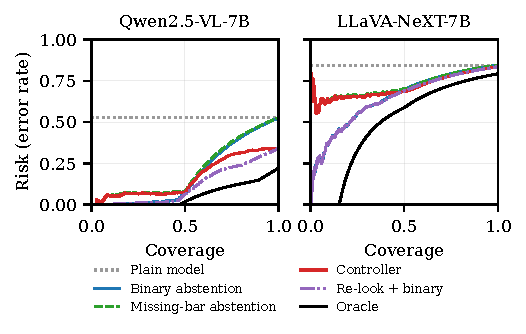
\includegraphics[width=\columnwidth]{figures/e5_risk_coverage.pdf}
\caption{TODO}
\label{fig:e5}
\end{figure}

% TODO (Naman): results (Table~\ref{tab:e5}, Figure~\ref{fig:e5}).
% Facts: results/e5.md tables and the per-class re-look breakdown.

% TODO (Naman): what the re-look actually fixes, and the oracle gap.
% Facts: results/e5.md, "Read these before writing them up", points 1 to 5.

\section{Discussion}
\label{sec:discussion}

% TODO (Naman): is the type separability hypothesis supported, now that E4 and
% E5 are in. Inputs: E3 (results/synth_type_probes.md,
% results/chartqa_type_probes.md), E4 and E5 above, and pilot 3 once Yash's
% probe results are in.
